\documentclass[10pt]{article}
\usepackage[utf8]{inputenc}
\usepackage[T1]{fontenc}
\usepackage{amsmath}
\usepackage{amsfonts}
\usepackage{amssymb}
\usepackage[version=4]{mhchem}
\usepackage{stmaryrd}
\usepackage{graphicx}
\usepackage[export]{adjustbox}
\graphicspath{ {./images/} }
\usepackage{fvextra, csquotes}

\begin{document}

    This problem explores some aspects of the two main methods of exoplanet detection: radial velocity and transit. Throughout this problem we shall consider a particular system of a single planet (P) in a circular orbit with radius $a$ around a solar-type star (S). We shall refer to this system as the "SP system".\\
    (D01.1) The V-band apparent magnitude of the star S is $7.65 \pm 0.03 \mathrm{mag}$, the parallax is $20.67 \pm 0.05$ milliarcsecond and the bolometric correction (BC) is -0.0650 mag. Thus the star has a higher bolometric luminosity than its V-band luminosity.
    
    Estimate the mass of the star, $M_{\mathrm{s}}$ (in units of $\mathrm{M}_{\odot}$ ), assuming a mass - luminosity ( $M-L$ ) relation of the form $L \propto M^{4}$. Also estimate the uncertainty in $M_{\mathrm{s}}$. You may need $\mathrm{d} \ln x / \mathrm{d} x=1 / x$.
    
    \section*{Radial Velocity method}
    The radial velocity method uses the Doppler shift $\delta \lambda \equiv \lambda_{\text {obs }}-\lambda_{0}$ between the observed wavelength $\lambda_{\text {obs }}$ and the rest wavelength $\lambda_{0}$ of a known spectral line to detect an exoplanet and determine its characteristics.
    
    The figure below shows the $\delta \lambda$ for the Fe I line $\left(\lambda_{0}=543.45 \times 10^{-9} \mathrm{~m}\right)$ as a function of time as observed for the SP system.\\
    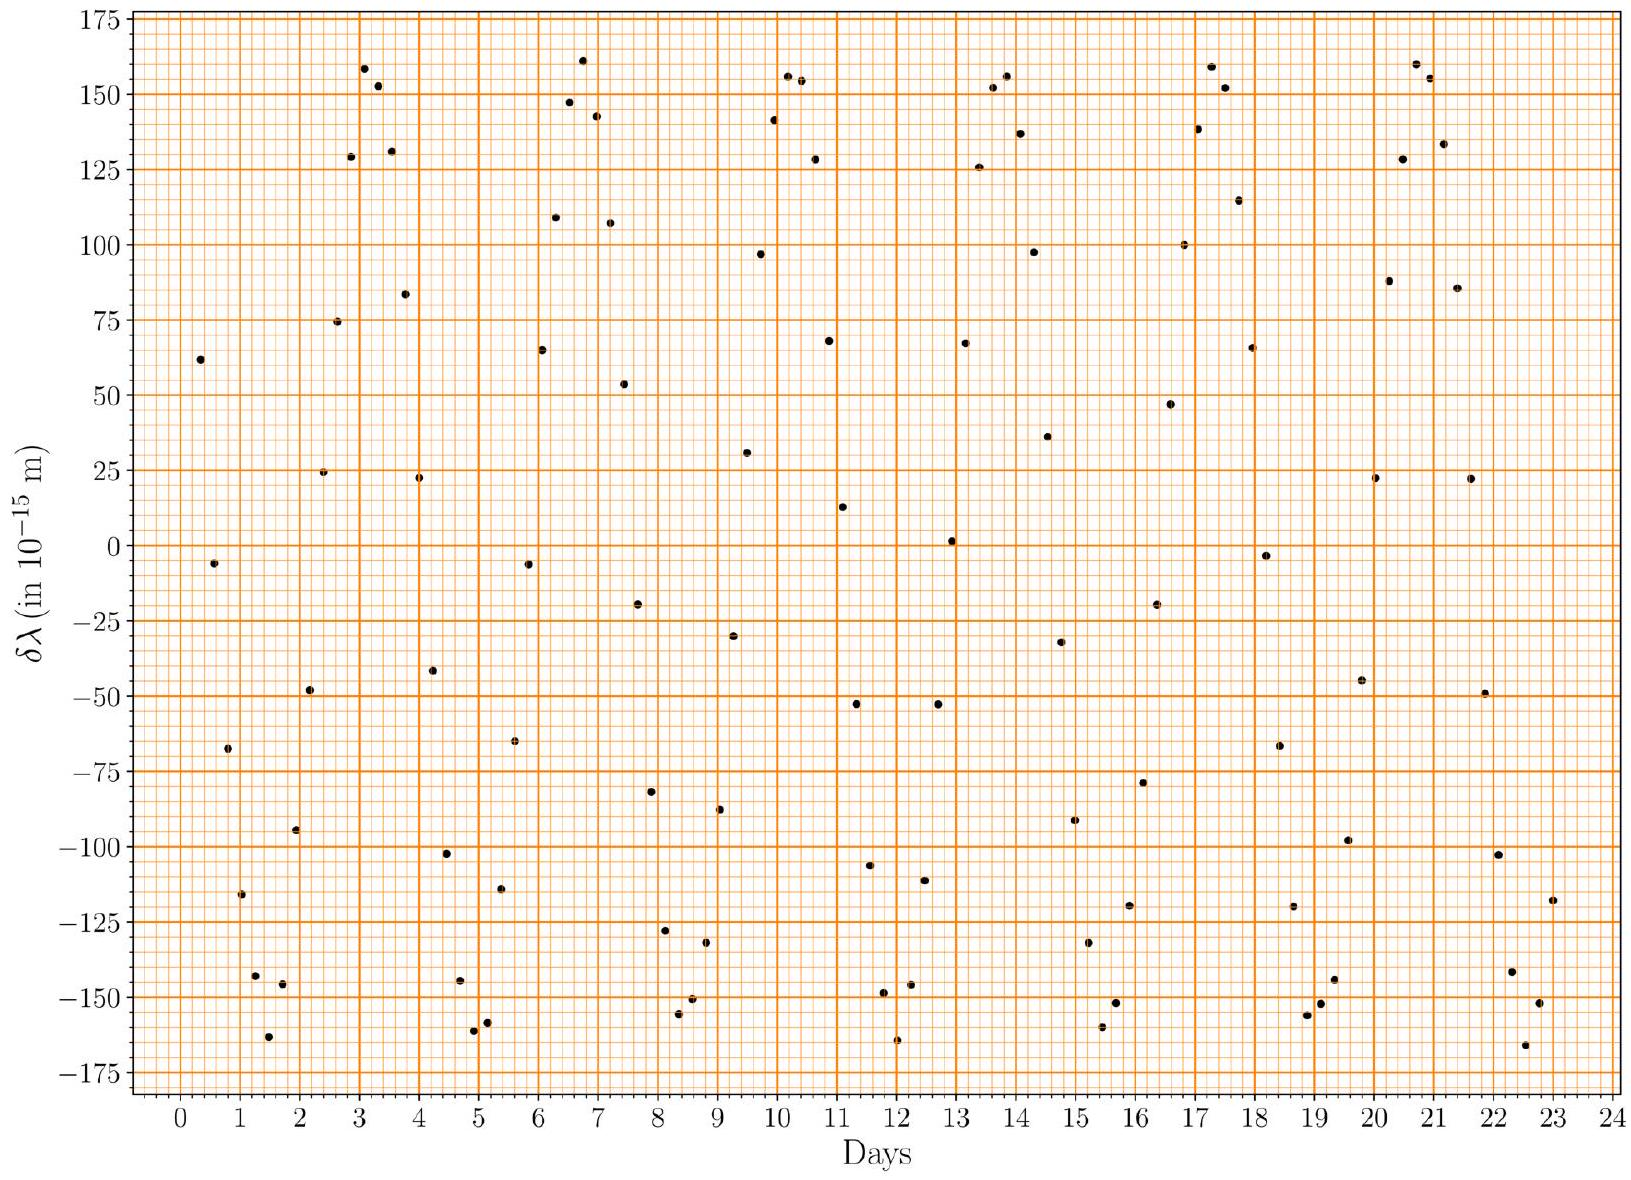
\includegraphics[max width=\textwidth, center]{2025_08_23_9a7c688c47c330d7bfc8g-1}
    
    The radial velocity semi-amplitude $K$ is defined as $K \equiv\left(v_{\mathrm{r}, \max }-v_{\mathrm{r}, \min }\right) / 2$ where $v_{\mathrm{r}, \max }$ and $v_{\mathrm{r}, \min }$ are the maximum and minimum radial velocities, respectively. For a circular planetary orbit the semi-amplitude $K$ can be written as:
    
    $$
    K=\left(\frac{2 \pi G}{T}\right)^{1 / 3} \frac{M_{\mathrm{p}} \sin i}{\left(M_{\mathrm{p}}+M_{\mathrm{s}}\right)^{2 / 3}}
    $$
    
    where $T$ is the period, $i$ is the inclination of the planetary orbit (angle between the normal to the orbital plane of the planet and the line of sight of the observer), $M_{\mathrm{p}}$ and $M_{\mathrm{s}}$ are the masses of the planet and the star, respectively.\\
    (D01.2) Use the above graph given in the Summary Answersheet (rotated by 90 deg ) to answer the following.\\
    (D01.2a) Draw a smooth curve associated with the observed data shown in the graph.\\
    (D01.2b) Select appropriate points on your drawn curve and use suitable methods to determine $T$ and $K$ along with respective uncertainties. All data points used for the calculation of $T$ and $K$ must be shown in the table in the Summary Answersheet. Use the rest of the Table to show your intermediate calculations, as needed, with appropriate headers.\\
    (D01.2c) Find the minimum mass of the planet $M_{\mathrm{p}, \min }$ (in $\mathrm{M}_{\odot}$ ), and its corresponding uncertainty assuming $M_{\mathrm{p}} \ll M_{\mathrm{s}}$.\\
    (D01.2d) Using the value of $M_{\mathrm{p}, \min }$ estimated in part (D01.2c), calculate the minimum value of the semi-major axis of the planet's orbit, $a_{\min }$, in au and its uncertainty.
    
    \section*{Transit method (without limb darkening)}
    The schematic diagram of a planet transit (not drawn to scale) is shown below. Initially, we shall assume the stellar disk to have a uniform average intensity with some intrinsic noise due to the star itself.\\
    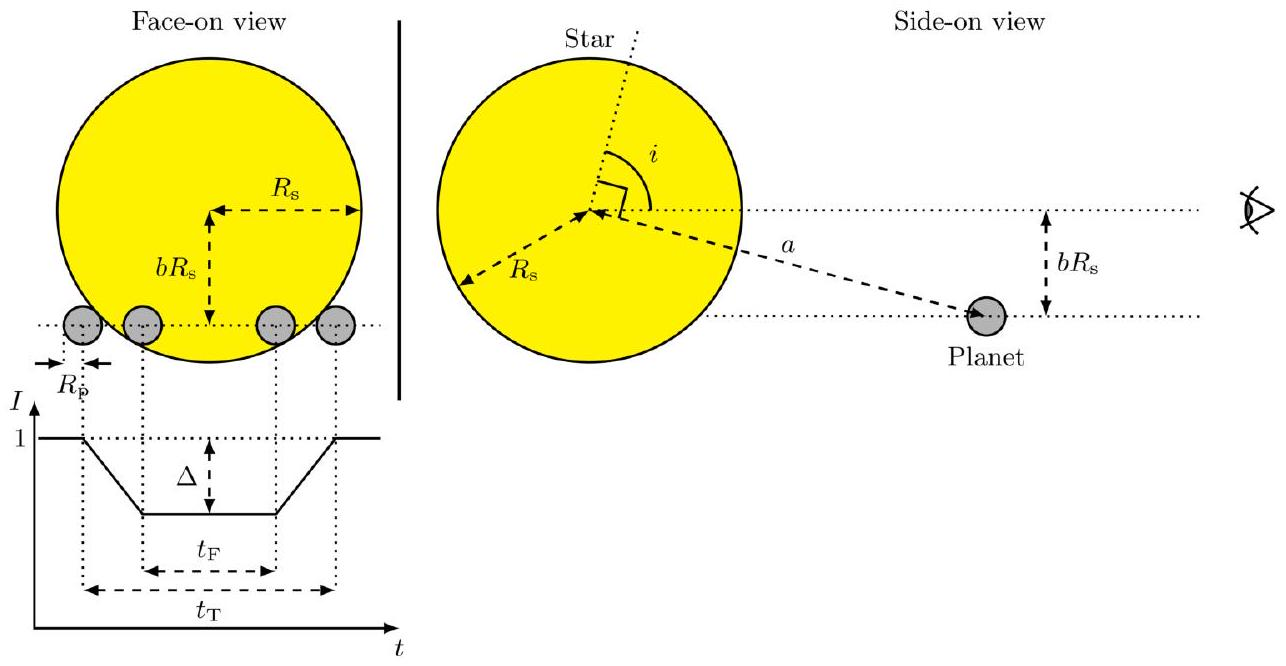
\includegraphics[max width=\textwidth, center]{2025_08_23_9a7c688c47c330d7bfc8g-2}
    
    The lightcurve of the normalized intensity, $I$, as a function of time $t$ is shown in the schematic diagram of the transit above. The average stellar intensity outside the transit is taken as unity. The maximum decrease in the intensity is given by $\Delta$ in the normalized light curve. For a uniformly bright stellar disk, the radius of the planet, $R_{\mathrm{p}}$, is related to $\Delta$ as
    
    $$
    \left(\frac{R_{\mathrm{p}}}{R_{\mathrm{s}}}\right)^{2}=\Delta,
    $$
    
    where $R_{\mathrm{s}}$ is the radius of the star.\\
    The total duration of transit (when part or all of the planet covers the stellar disk) is given by $t_{\mathrm{T}}$, while $t_{\mathrm{F}}$ gives the duration when the planet is fully in front of the stellar disk. The "impact parameter" $b$ is the projected distance between the planet and centre of the stellar disk at the mid-point of the transit, in units of the stellar radius, $R_{\mathrm{s}}$.
    
    For a nearly edge-on star-planet orbit, the impact parameter is given by the formula
    
    $$
    b=\left[\frac{(1-\sqrt{\Delta})^{2}-\left(t_{\mathrm{F}} / t_{\mathrm{T}}\right)^{2}(1+\sqrt{\Delta})^{2}}{1-\left(t_{\mathrm{F}} / t_{\mathrm{T}}\right)^{2}}\right]^{1 / 2}
    $$
    
    Data Analysis Examination\\
    (D01.3) For the SP system, the stellar radius is known to be $R_{\mathrm{s}}=1.20 R_{\odot}$, and the transit of the planet is indeed visible. Using the minimum orbital radius, $a_{\min }$, estimated in part ( $D 01.2 \mathrm{~d}$ ), find the minimum value, $i_{\text {min }}$, of the inclination angle.
    
    Assuming a stellar disk of uniform brightness, the transit lightcurve would look like as shown below.\\
    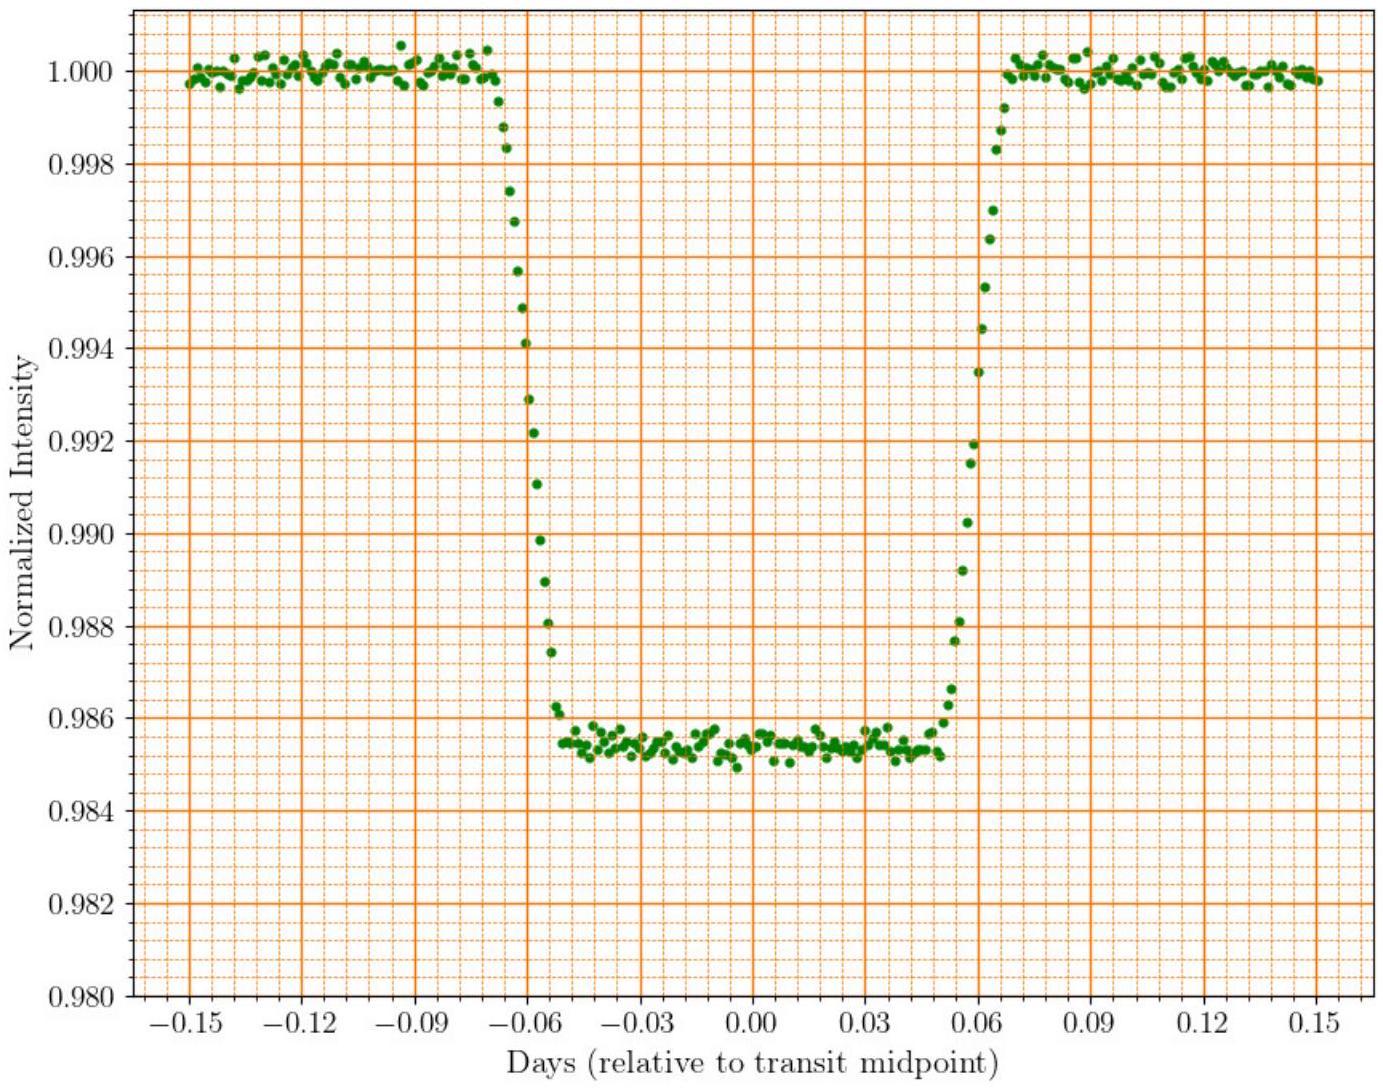
\includegraphics[max width=\textwidth, center]{2025_08_23_9a7c688c47c330d7bfc8g-3}\\
    (D01.4) Using the given lightcurve answer the following questions. For your reference the above lightcurve is also given in the Summary Answersheet.\\
    (D01.4a) Estimate the values of $t_{\mathrm{T}}$ and $t_{\mathrm{F}}$ in days by marking appropriate readings on the graph.\\
    (D01.4b) Estimate the mean value of $\Delta$ by marking appropriate readings on the graph and hence find $R_{\mathrm{p}}$ in units of $\mathrm{R}_{\odot}$.\\
    (D01.4c) Determine the value of $i$ in degrees assuming the orbital radius to be $a_{\min }$.
    
    \section*{Introducing limb darkening}
    So far we have assumed the stellar disk to be uniformly bright. In reality, the observed brightness of the stellar disk is not uniform due to "limb darkening" - an optical effect where the central part of the stellar disk appears brighter than the edge, or the "limb".
    
    The limb darkening effect can be measured by the relative intensity $J(\theta) \equiv \frac{I(\theta)}{I(0)}$, where $\theta$ is the angle between the normal to the stellar surface at a point and the line joining the observer to that point, $I(\theta)$ is the observed intensity of the stellar disk at that point ( $I(0)$ being the intensity at the centre of the stellar disk). For a distant observer, $\theta$ varies from $\theta=0$ (centre of the disk) to $\theta \approx 90^{\circ}$ )(edge of the disk).
    
    Data Analysis Examination\\
    (D01.5) The table below gives measured $J(\theta)$ at a certain wavelength for the Sun. We shall assume that the same limb darkening profile holds for the star S .
    
    \begin{center}
    \begin{tabular}{|c|c|c|c|c|c|c|c|}
    \hline
    $\theta$ & $J(\theta)$ & $\theta$ & $J(\theta)$ & $\theta$ & $J(\theta)$ & $\theta$ & $J(\theta)$ \\
    \hline
    $0^{\circ}$ & 1.000 & $20^{\circ}$ & 0.971 & $40^{\circ}$ & 0.883 & $70^{\circ}$ & 0.595 \\
    \hline
    $10^{\circ}$ & 0.994 & $25^{\circ}$ & 0.950 & $50^{\circ}$ & 0.794 & $80^{\circ}$ & 0.475 \\
    \hline
    $15^{\circ}$ & 0.984 & $30^{\circ}$ & 0.943 & $60^{\circ}$ & 0.724 & $90^{\circ}$ & 0.312 \\
    \hline
    \end{tabular}
    \end{center}
    
    The limb darkening profile can be modelled by a quadratic formula:
    
    $$
    J(\theta)=1-a_{1}(1-\cos \theta)-a_{2}(1-\cos \theta)^{2},
    $$
    
    where $a_{1}$ and $a_{2}$ are two constants.\\
    We shall estimate the unknown coefficients $a_{1}$ and $a_{2}$ from the given data by making a plot with suitable variables.
    
    \begin{displayquote}
    (D01.5a) Choose a pair of variables $\left(x_{1}, y_{1}\right)$ which are suitable functions of $\theta$ and $J$, that you want to plot along $x$ and $y$ axes, respectively, to determine $a_{1}$ and $a_{2}$. Write the expressions for $x_{1}$ and $y_{1}$.
    \end{displayquote}
    
    If you need to define additional variables for additional plots, define them as $\left(x_{2}, y_{2}\right)$, etc.\\
    (D01.5b) Tabulate the values necessary for your plots.\\
    (D01.5c) Plot the newly defined variables on the given graph paper (mark your graph as "D01.5c").\\
    (D01.5d) Obtain $a_{1}$ and $a_{2}$ from the plot. Uncertainties on the values are not needed.
    
    \section*{Transit in the presence of limb darkening}
    Now, we consider planetary transits across a limb darkened stellar disk. In the presence of limb darkening, which we shall model by the quadratic formula of $J(\theta)$ given above, the average observed intensity of the entire stellar disk (without any transit), $\langle I\rangle$, is given by:
    
    $$
    \langle I\rangle=\left(1-\frac{a_{1}}{3}-\frac{a_{2}}{6}\right) I(0)
    $$
    
    Further, the dip in the light caused by the transiting planet now depends not only on the relative size of the planet and the star, $\left(\frac{R_{\mathrm{p}}}{R_{\mathrm{s}}}\right)$, but also on the intensity profile of the stellar disk along the transit chord, which in turn, depends on the angle of inclination, $i$.
    
    The schematic diagram below (not drawn to scale) shows the configuration. Note that the brighter part of the star is shown in a darker shade, while the planet is shown as a black dot.\\
    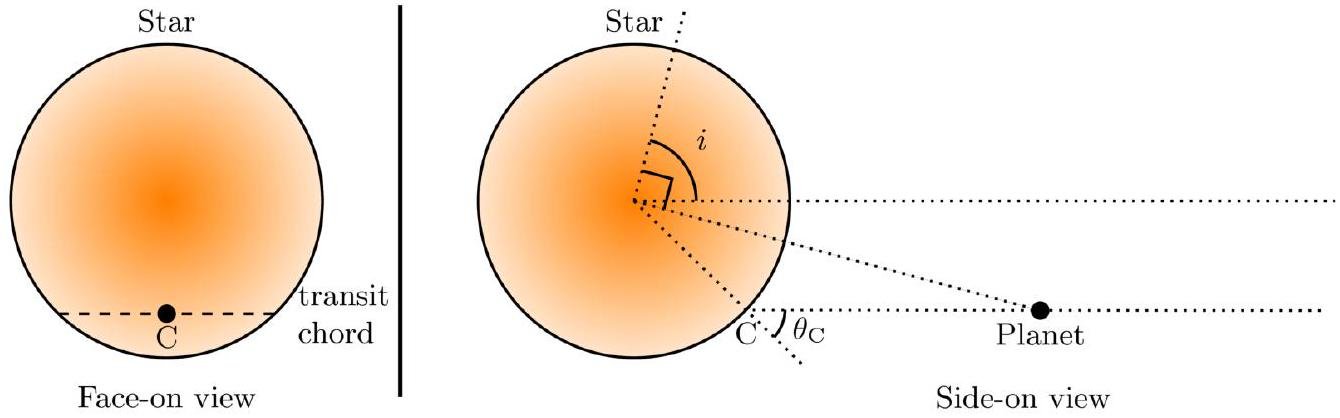
\includegraphics[max width=\textwidth, center]{2025_08_23_9a7c688c47c330d7bfc8g-4}
    
    Here the relation between $\left(\frac{R_{\mathrm{p}}}{R_{\mathrm{s}}}\right)$ and the measured $\Delta$ from the light curve is
    
    $$
    \Delta=\frac{I\left(\theta_{\mathrm{C}}\right)}{\langle I\rangle}\left(\frac{R_{\mathrm{p}}}{R_{\mathrm{s}}}\right)^{2},
    $$
    
    where $I\left(\theta_{\mathrm{C}}\right)$ is the intensity of the stellar disk at the midpoint of the transit chord (point C in the figure above), $\theta_{\mathrm{C}}$ being the angle between the line of sight and the normal to the surface at that point. From the above it is obvious that for a given star, the same value of $\Delta$ can be produced by many combinations of the planet size, $R_{\mathrm{p}}$, and the inclination angle $i$.\\
    (D01.6) It is possible to uniquely determine both $R_{\mathrm{p}}$ and $i$ by using data from transit lightcurves at two wavelengths, say, $\lambda_{\mathrm{B}}$ (blue) and $\lambda_{\mathrm{R}}$ (red). The limb darkening coefficients for these two wavelengths are given below:
    
    \begin{center}
    \begin{tabular}{|c|c|c|}
    \hline
    Wavelength & $a_{1}$ & $a_{2}$ \\
    \hline
    $\lambda_{\mathrm{B}}$ & 0.82 & 0.05 \\
    \hline
    $\lambda_{\mathrm{R}}$ & 0.24 & 0.20 \\
    \hline
    \end{tabular}
    \end{center}
    
    (D01.6a) Choose the correct statement among the following that describes the relation between the maximum depth of the transit $\Delta$ for $\lambda_{\mathrm{B}}$ and the inclination angle $(i)$ of the orbit and tick it ( $\boldsymbol{\checkmark}$ ) in the Summary Answersheet.\\
    A. $\Delta$ increases with decreasing $i$.\\
    B. $\Delta$ decreases with decreasing $i$.\\
    C. $\Delta$ is independent of $i$.\\
    (D01.6b) The maximum depth of the transit ( $\Delta$ ) for the "SP system" was measured to be 0.0182 and 0.0159 for $\lambda_{\mathrm{B}}$ and $\lambda_{\mathrm{R}}$, respectively.
    
    Draw schematic transit light curves for both $\lambda_{\mathrm{B}}$ and $\lambda_{\mathrm{R}}$ on the given grid and label the curves by "B" and "R", respectively. Assume that the total transit duration is same for both wavelengths. The curves need not be to scale, but should represent the shapes of the light curves correctly.\\
    (D01.7) We shall use a graphical method to find the values of $R_{\mathrm{p}}$ and $i$ for the SP system using the measurements of $\Delta$ at $\lambda_{B}$ and $\lambda_{R}$.\\
    (D01.7a) Write an appropriate expression connecting the relevant variables that are to be plotted.\\
    (Hint: You may consider $i$ or $b$, and $R_{\mathrm{p}}$, among the relevant variables.)\\
    (D01.7b) Tabulate the appropriate quantities that are to be plotted.\\
    (D01.7c) Draw a suitable graph and mark it as "D01.7c".\\
    (D01.7d) Estimate the values of $R_{\mathrm{p}}$ (in $\mathrm{R}_{\odot}$ ) and $i$ (in degrees) from the graph.\\
    (D01.8) Based on the results obtained in this problem, indicate whether the planet P is "ROCKY" or "GASEOUS" by ticking $(\checkmark)$ the appropriate box in the Summary Answersheet.

\end{document}